\documentclass[crop,tikz]{standalone}


\usepackage{standalone}

\usepackage{times}
\usepackage{latexsym}
\usepackage{linguex} 
% Tikz
\usepackage{tikz}
\usepackage{pgf}
\usetikzlibrary{shapes,external}
\usetikzlibrary{shapes.multipart}
\usetikzlibrary{calc}

% Math
\usepackage{amsmath}
\usepackage{amssymb}
\usepackage{mathtools}
\usepackage{proof}

% Decorated Arrow
\newlength{\arrow}
\settowidth{\arrow}{\scriptsize$10$}
\newcommand*{\myrightarrow}[1]{\xrightarrow{\mathmakebox[\arrow]{\text{\scriptsize #1}}}}

% Color defs
\usepackage{xcolor}
\definecolor{first}{RGB}{82,82,82}
\definecolor{enc}{RGB}{253,192,134}
\definecolor{dec}{RGB}{127,201,127}
\definecolor{dec2}{RGB}{140,220,140}
\definecolor{emb}{RGB}{190,174,212}
\definecolor{methods}{RGB}{140,22,22}


% graphs
\usepackage{float}
\usepackage{subcaption}
\usepackage{graphicx}

% Tabular
\usepackage{tabularx}
\usepackage{booktabs}
\newcolumntype{m}{>{\hsize=.65\hsize}X}
\newcolumntype{s}{>{\hsize=.4\hsize}c}
\newcolumntype{u}{>{\hsize=.25\hsize}X}
\usepackage{multicol}
\usepackage{multirow}


\usepackage{url}

\begin{document}

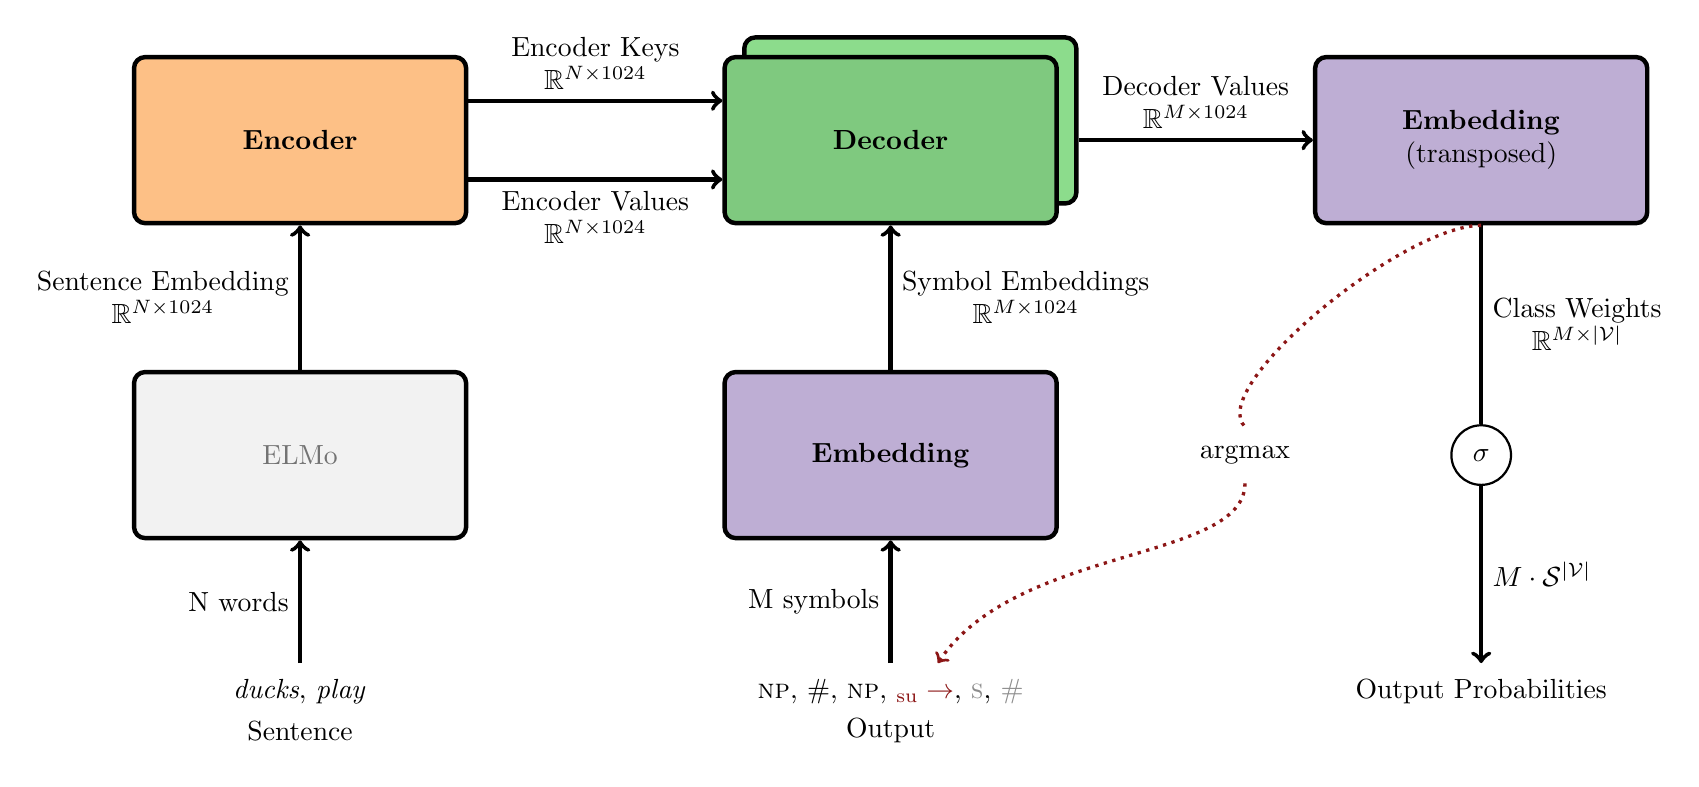
\begin{tikzpicture}[every text node part/.style={align=center},
 every node/.style={transform shape},
 scale=1,
block/.style={rectangle, inner sep=0pt, minimum width=120pt, minimum height=60pt, rounded corners, ultra thick},
str/.style={rectangle, inner sep=0pt, minimum width=120pt, minimum height=20pt},
arrow/.style={->, ultra thick},
pwise/.style={circle, inner sep=0pt, minimum size=10pt},
smallblock/.style={circle, inner sep=5pt, minimum size=12pt, rounded corners, thick}]


    \node[str] (stuff) at (0, 4.5) {Sentence};		
	\node[str] (sentence) at (0, 5) {\textit{ducks}, \textit{play}};		
	\node[str] (stuff2) at (7.5, 4.5) {Output};
	\node[str] (symbols) at (7.5, 5) {\textsc{np}, \#, $\textsc{np}$,  ${\color{methods}_\text{su}\to}$, ${\color{gray!90}\textsc{s}}$, ${\color{gray!90}\#}$};

	\node[block, draw=black, fill=gray!10] (elmo) at (0,8) {\textcolor{gray!110}{ELMo}};
	\node[block, draw=black, fill=enc] (te) at (0,12) {\textbf{Encoder}};
	\node[block, draw=black, fill=emb] (se) at (7.5,8) {\textbf{Embedding}};
	\node[block, draw=black, fill=dec2] (td2) at (7.75, 12.25) {};
	\node[block, draw=black, fill=dec] (td) at (7.5,12) {\textbf{Decoder}};
	\node[block, draw=black, fill=emb] (set) at (15,12) {\textbf{Embedding}\\ (transposed)};	
	\node[smallblock, draw=black] (ss) at (15, 8) {$\sigma$};
	\node[str, draw=white] (am) at (12, 8) {argmax};
	\node[str] (out) at (15,5) {Output Probabilities};	
	

	\draw (symbols) edge [arrow] node[left] {M symbols} (se);
	\draw  (sentence) edge [arrow] node[left] {N words} (elmo);
	\draw  (elmo) edge [arrow] node[left] {Sentence Embedding\\ $\mathbb{R} ^ {N \times 1024}$} (te);
	
	\draw  (se) edge [arrow] node[right] {Symbol Embeddings\\ $\mathbb{R} ^ {M \times 1024}$} (td);
	\draw ($(te.east) + (0, 0.5)$) edge [arrow] node[above] {Encoder Keys\\ $\mathbb{R}^ {N \times 1024}$} ($(td.west) + (0, 0.5)$);
	\draw ($(te.east) + (0, -0.5)$) edge [arrow] node[below] {Encoder Values\\ $\mathbb{R}^ {N \times 1024}$} ($(td.west) + (0, -0.5)$);\
	\draw ($(td.east) + (0.25, 0)$) edge [arrow] node[above] {Decoder Values\\ $\mathbb{R}^ {M \times 1024}$} (set);
	\draw (set) edge [ultra thick] node[right] {Class Weights \\
	    $\mathbb{R}^{M \times |\mathcal{V}|}$}(ss);
	\draw (ss) edge [arrow] node[right] {$M \cdot \mathcal{S}^{|\mathcal{V}|}$} (out);
	\draw (set.south) [dotted, very thick, color=methods] .. controls +(-1,0) and +(-0.5, 0.5) .. (am.north);
	\draw (am.south) [dotted, very thick, ->, color=methods] .. controls +(0,-1) and +(1, 1.5) .. ($(symbols.north) + (0.6,0)$);
\end{tikzpicture}

\end{document}